\documentclass[12pt]{article}

\usepackage[utf8]{inputenc}    
\usepackage[T1]{fontenc}
\usepackage[francais]{babel}
\usepackage{graphicx}    

\title{\textbf{Projet d'électronique: Rapport préliminaire}}
\author{Dodeur Th. , Duchêne M. , Muteba J-L , Lambin C.}
\date{3 mars 2017} 

\begin{document}
\maketitle

\section{Objectifs}
	Réaliser une carte électronique centrée autour d'un microcontrôleur. Le rôle de cette carte sera de définir si la température d'une pièce
	dépasse une limite préalablement définie, et d'émettre une alarme le cas échéant. Pour ce faire, la carte sera notamment composée :
	\begin{itemize}
		\item d'un microcontrôleur (PIC 18f458) qui recevra des inputs, les traitera, et enverra les réponses sur les outputs adéquats
		\item d'une sonde de température (LM35), qui enverra la température au PIC sous forme d'un signal analogique
		\item de 2 afficheurs 7 segments qui afficheront en temps réel la température ressentie par la sonde
		\item d'une LED verte active tant que la température est en dessous de la limite
		\item d'une LED rouge qui clignotera tant que la température ne sera pas en dessous de la limite
	\end{itemize}
	L'état de la carte sera interfacé à l'aide d'une application Java, et le PIC sera programmé en C.	

\section{Cahier des charges}
	La carte sera capable :
	\begin{itemize}
		\item d'afficher la température
		\item d'émettre en permanence une lumière verte quand la température est acceptable, et une lumière rouge clignotante le cas échéant
		\item d'écouter l'interface Java via un port particulier et de réagir en conséquence
	\end{itemize}	
	L'interface Java permettra de communiquer avec la carte via le port RS232 d'un PC, et sera capable :
	\begin{itemize}
		\item de régler la température limite
		\item de visualiser l'état de la carte (température ambiante, alerte, etc...)
	\end{itemize}

\section{État d'avancement général}
	À ce jour, le schéma de la carte est complet et définitif, le code C permet au PIC de recevoir les informations de la sonde et
	d'afficher la température, l'interface Java basique sera bientôt implémentée.

\section{Répartition du travail}
	Toute la partie électronique a été implémenté par Lambin Cédric, le code C et la simulation sont gérer par Duchêne Maxime, 
	tandis que la programmtion Java est assurée par Dodeur Thanh Son et Muteba Jean-Luc.
	
\section{Schéma complet et définitif de la carte}
	\textit{voir annexe A}

\appendix
\newpage

\part*{Annexe}

\section{Dessin de la carte}
	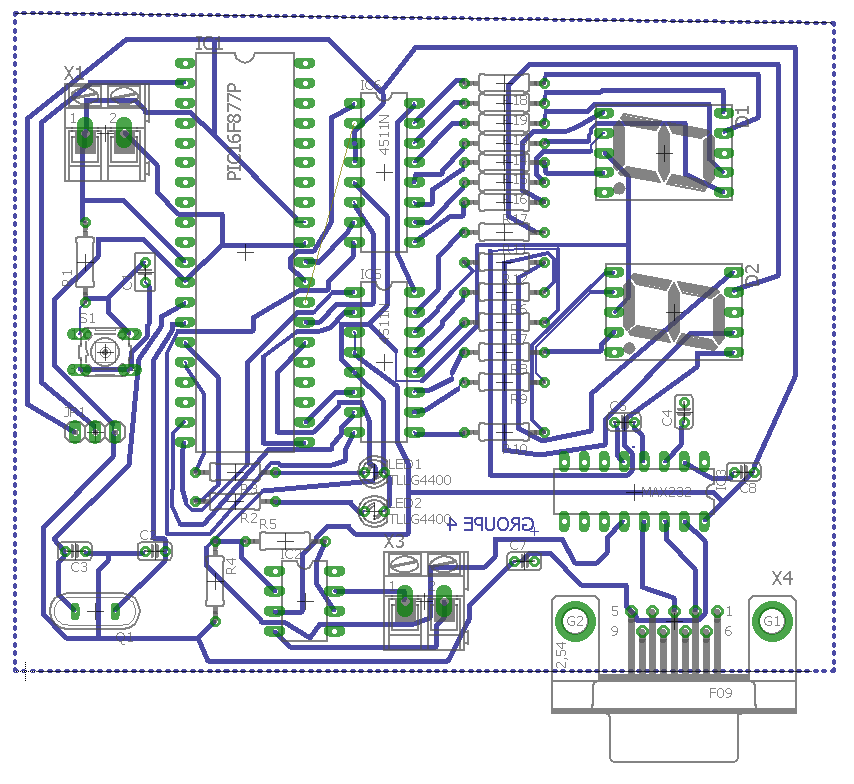
\includegraphics[scale=0.4]{17360818_804944499659683_173090360_n.png}
    \newpage
	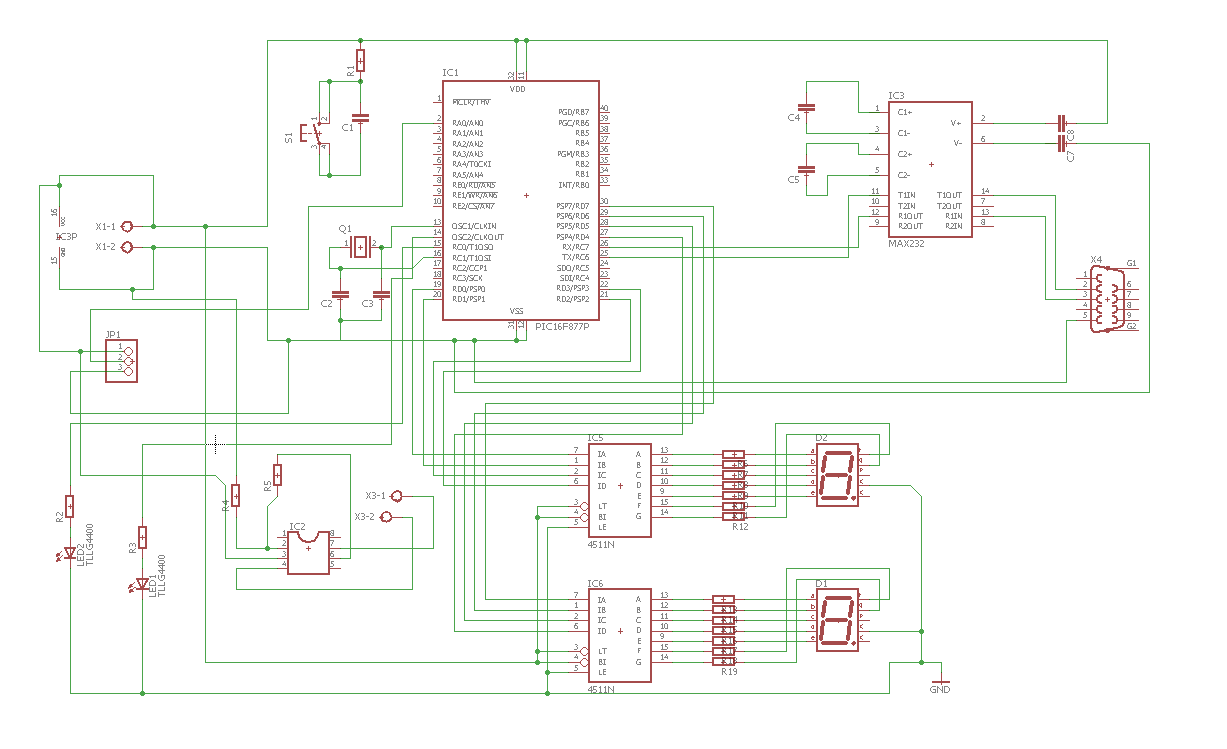
\includegraphics[scale=0.7]{17310461_804699796350820_1466488599_o.png}
\end{document}